\subsection{Prime Time Ratio}
\label{subsec:primetime}

In section ~\ref{sec:methodology}, we established the importance of measuring behavior during prime time hours. To reiterate, the prime time hours as defined by the FCC is the period between 7:00 PM -- 11:00 PM on weeknights when the network is under peak load~\cite{fcc2014measuring-broadband}. \todo{The first occurrence of this definition was ... should this be in methodology?? }

Our analysis of the peak usage in figure~\ref{fig:TS-data-rate-daily} motivated us to revisit this definition. We observed that in our dataset the four hour period 8:00 PM -- 12:00 AM is a much better indicator of prime-time hours than the FCC's original definition. This discrepancy could be limited to high tier households only, or it could imply that due to the flexibility of video-on-demand, consumers across the country are opting for a later time to watch real-time-entertainment. 

\begin{figure}[ht!]
\begin{minipage}{\linewidth}
\centering
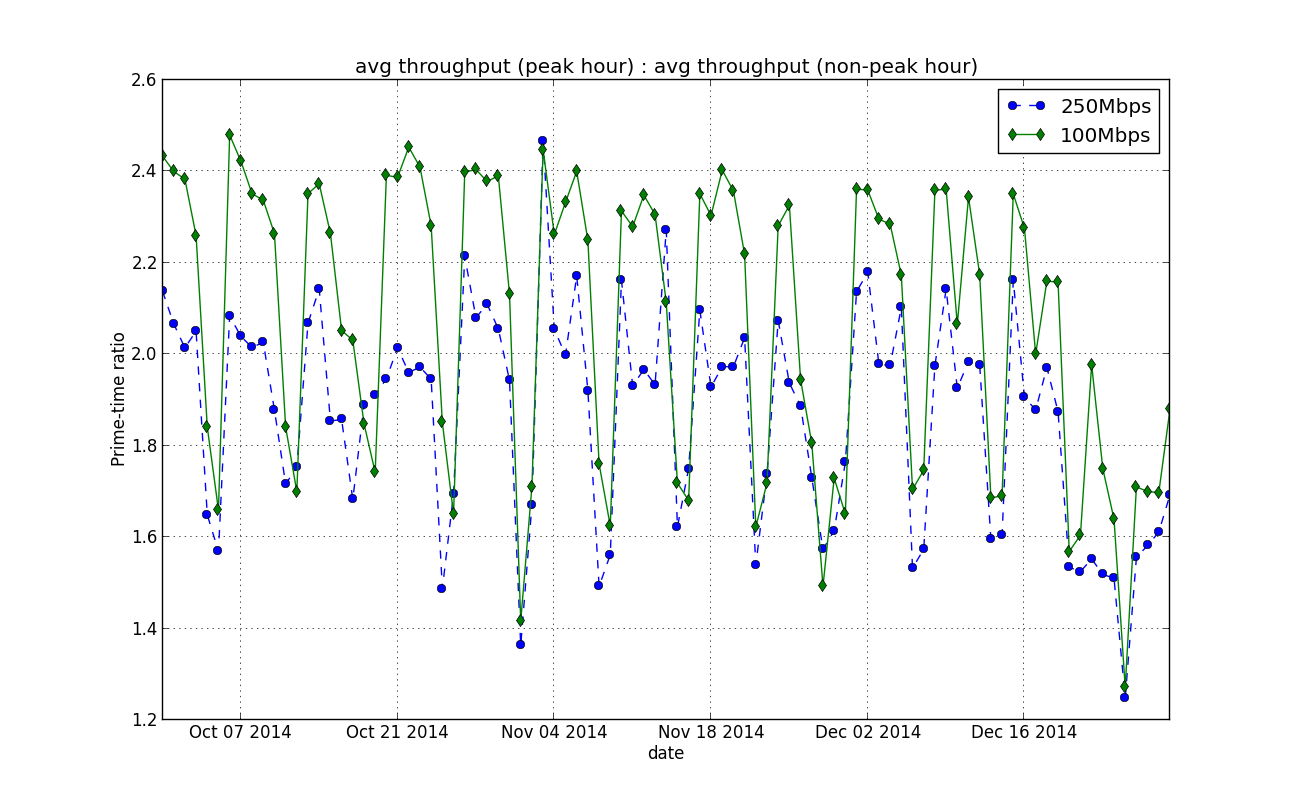
\includegraphics[width=\linewidth]{figures/prime-time-ratio-by-date[replace].png}
\caption{Prime Time ratio showing weekly pattern + differences during holiday periods (Thanksgiving, Christmas)}
%http://riverside.noise.gatech.edu:8083/separated/full/prime-time-ratio-by-date.png
\label{fig:TS-prime-time-ratio}
\end{minipage}
\end{figure}

We use the updated definition of prime-time (as 8:00 PM -- 12:00 AM) to examine the aggregate prime-time ratio each day for both \test and \control sets. Figure ~\ref{fig:TS-prime-time-ratio} shows that the prime-time ratio for the \test set is 10\% less than the control set, implying that the ratio of average data rates in peak (prime-time) hours and off-peak hours in a day reduces due to the capacity upgrade from 105 Mbps to 250 Mbps. The prime-time ratio can decrease only in two scenarios (1) the usage during prime time decreases, and off-peak remains the same, or (2) the usage during off-peak hours increased due to the upgrade.

%measures the variance in prime-time hours and off-peak hours
We also noticed that multiple agencies define prime-time differently causing difficulty in comparing studies. We recommend that the FCC studies prime-time usage behavior and standardizes its definition. If supported by analysis, the FCC should update prime-time to a later hour.%Another definition might be local to each agent examining their peak network load as the approx time when aggregated traffic is 90\%-ile of the maximum load, which can cause latency delays. \todo{ should this be in the discussion instead }
